\documentclass{article}
\usepackage{graphicx}
\usepackage{geometry}                % See geometry.pdf to learn the layout options. There are lots.
\geometry{letterpaper}
\usepackage{amssymb}
\usepackage{amsthm}
\usepackage{epstopdf}
\usepackage[utf8]{inputenc}
\usepackage[usenames,dvipsnames]{color}
\usepackage[table]{xcolor}
\usepackage{hyperref}
\graphicspath{ {./images/} }
\usepackage{wrapfig}


\newcommand{\projectname}{Digital Door Sign}
\newcommand{\productname}{Digital Door Sign}
\newcommand{\projectleader}{G.S. Panturu}
\newcommand{\documentstatus}{Ready}
%\newcommand{\documentstatus}{Submitted}
%\newcommand{\documentstatus}{Released}
\newenvironment{explanation}{%
   \color{black}
}{}
\newcommand{\version}{0.5}

\begin{document}

\begin {center}
{\Huge Project Proposal} \\[3em]
{\LARGE \productname} \\[3em]
\date{October 2019}
\begin{tabular}{|l|l|}
\hline
Project Name & \projectname \\ \hline
Project Leader & \projectleader \\ \hline
Document state & \documentstatus \\ \hline
Version & \version \\ \hline
\end{tabular}
\end{center}
\pagebreak
\tableofcontents

\pagebreak
\section{Revisions}
\begin{tabular}{|l|l|l|}
\hline
\cellcolor[gray]{0.5}\textcolor{white}{Date} & \cellcolor[gray]{0.5}\textcolor{white}{Author} & \cellcolor[gray]{0.5}\textcolor{white}{Change} \\ \hline
23.09.2019&G.S.P/F.B./B.C./J.H.&Initial Situation added \\ \hline
27.09.2019&G.S.P/F.B./B.C./J.H.& Introduction added \\ \hline
5.10.2019&G.S.P/F.B./B.C./J.H.&Infosabout special rooms \\ \hline
7.10.2019&G.S.P/F.B./B.C./J.H.& Girls' Day and Open Doors Day Views examples created\\ \hline
8.10.2019&F.B./B.C./J.H.&Updated views examples added \\ \hline
10.10.2019&/F.B./B.C./J.H.&Changes made by Mr. Bauer added \\ \hline
14.10.2019&G.S.P/F.B./B.C./J.H.&Updated special rooms\\ \hline
17.10.2019&G.S.P/F.B./B.C./J.H.&Added workshop room infos\\ \hline
24.10.2019&G.S.P/F.B./B.C./J.H.& Correction and Latex final version \\ \hline
\end{tabular}
\pagebreak
\section{Introduction}
\begin{explanation}
The technical college in Leonding (Upper Austria) is a high school with four departments: 
\begin{itemize}
  \item Informatics
  \item Media technology
  \item Medicine technology
  \item Electronics
\end{itemize}
Our school has over 1000 students and over 100 teachers.\\
For a technical college is very important to have a modern design. In the last few years our school has been renovated outside and some rooms on the inside.\\
It is also very important to be up to date with new technologies that can be used in buildings, that can let our school look more modern and can let people find rooms easier, especially during open-door days for new pupils and people interested in our school. \\
That’s why we want to start using a digital signage system which lets people see which rooms are being used and which not, when and where events like tests or seminars are taking place.\\
This project is based on two preliminary projects, one using tablets as digital door signs and one using E-Papers.
\end{explanation}
\pagebreak

\section{Initial Situation}

\begin{wrapfigure}{r}{0.25\textwidth} %this figure will be at the right
    \centering
     \caption{Classroom}
    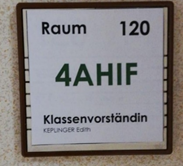
\includegraphics[width=0.25\textwidth]{images/klassenraum_alt.png}
    \caption{Computer room}
    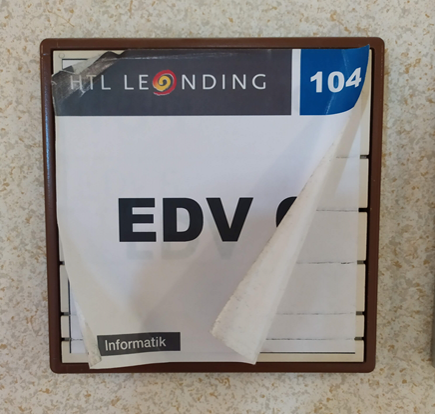
\includegraphics[width=0.25\textwidth]{images/edv.png}
   \caption{Workshop rooms}
    \includegraphics[width=0.35\textwidth]{images/werkstatt_alle.png}
\end{wrapfigure}
\vspace{1.2cm}

\begin{explanation}
There are different types of rooms in our school. Each room is tagged by a sheet of paper telling different information, depending on the room type.\\
The most common room types are:
departments: 
\begin{itemize}
  \item	Classrooms \\
  \\
  These rooms’ signage contains the room number, the main class that is usually in there and the form teacher.
  \item Computer rooms \\
  \\
  The computer rooms’ signage currently contains only the room number, the computer room’s name and the room’s department (e.g. informatics). The schedule is pinned on the door.
  \item	Teachers’ rooms \\
  \\
  These rooms have multiple teachers with their name and picture.
  \item	Special purpose rooms \\
  \\
  The physics and chemistry rooms are used for lessons in these subjects. Furthermore, they are sometimes used as special rooms for holding tests.
  \item	Assembly hall \\
  \\
  This room is used for the final exams and special events.
  \item	Workshops \\
  \\
  These rooms have a different signage compared to the classrooms. They only contain the room number and the room name. Some of them have symbols for the rules that have to be followed (e.g. wearing work clothing or safety glasses). Other rooms have a special schedule that is divided in morning and afternoon lessons. 
  \item	Meeting room (E26, ILB, …) \\
  \\
  Rooms with no regular schedule, booked for single events.
  \\
\end{itemize}

Currently all our rooms and events do not have a concrete signage showing which events are currently taking place. Even worse, one may not rely on the regular schedule shown at the doors.\\
Moreover, it happens that teachers spontaneously need a computer room, a special purpose room, a workshop, etc. for their lessons. Searching for one in WebUntis is time-consuming and knocking at all the room door to see if the room is occupied is pretty disturbing during regular lessons, not to mention situations where tests or exams take place. 
\end{explanation}
\pagebreak

\section{General Conditions and Constraints}

\begin{explanation}
\textbf{Our know-how:}
\begin{itemize}
\item Java 
\item Angular
\item mySQL 
\item C++
\\
\end{itemize}
There are two different prototypes available from preceding projects: one using tablets and another using E-Paper devices. 
\\We can cooperate with two other teams that worked on the previous versions of this project. Both projects aren’t finished yet. Furthermore, the final outcome of this project is not defined yet. E-Paper devices and tablets have a different backend, which has to be merged in order to combine both projects. \\
\\
Furthermore, these services have to be used:
\begin{itemize}
\item WebUntis – currently the regular schedule plus some of the extra events are planned/maintained in WebUntis. Unfortunately, the extra events are not completely planned in WebUntis (e.g. the final exams are rarely scheduled since they always take place in the same rooms). First investigations have shown that the clumsy user interface for entering events is the reason why teachers hardly ever schedule their extra events, nevertheless this tool plays a central role in scheduling of courses and events at the HTL and has to be part of a future solution for a digital signage. 
\item WebUntis API: WebUntis offers a sort of user interface to the internal data model. In order to integrate WebUntis into our new system this API has to be used.
\\
\end{itemize}
\end{explanation}

\pagebreak

\section{Project Objectives and System Concepts}

\begin{explanation}
The content of the door signs depends on the situation whether the room is part of a special event or not. Most of the rooms have a regular schedule and serve the lectures and courses. In case of special events (FIT, Open Doors Day, …) the purpose may change and, therefore, the content of the digital door signs also has to change.\\
\\
\textbf{Computer rooms} \\
\\
The door sign at the IT-Rooms will display in addition to the room number and the weekly schedule events currently happening.\\
The physics/chemistry rooms can also be considered as an IT room since we want to display the weekly schedule.\\
\\
\textbf{Teacher rooms} \\
\\
The teacher’s sign will display every teacher located in the room, their name, their current location (or if they’re not having any lessons at the time) and the consultation hours of each teacher.\\
\\

\begin{wrapfigure}{r}{0.25\textwidth}
    \centering
    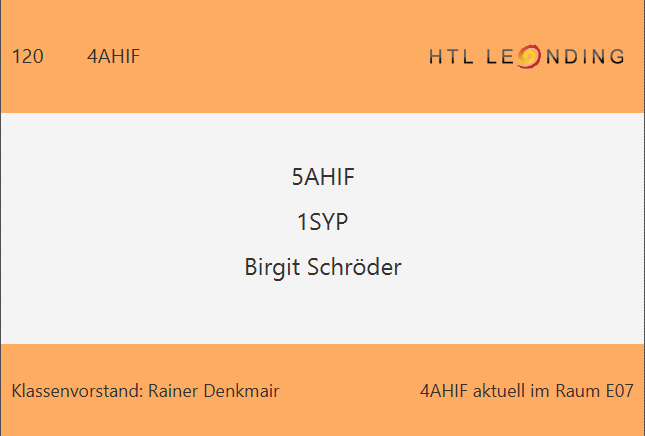
\includegraphics[width=0.45\textwidth]{images/views_examples/klassenview_normal.PNG}
    \caption{Classroom view - example}
\end{wrapfigure}


\textbf{Classrooms} \\
\\
The classroom signs will display 

\begin{itemize}
\item the room number, 
\item the main class and its form teacher,
\item the current location of the main class (if anywhere else), 
\item the current class in that room, 
\item the current subject, 
\item the current teacher,
\item special sign during an exam and
\item when the class is split it shows the room where the rest of the class currently is.
\end{itemize}

\newpage

\textbf{Workshop rooms} \\
\\
These rooms have different names like “Hochfrequenz- und Nachrichtentechnik”. These names must be displayed along with the room number. Furthermore, symbols for the rules that have to be followed (e.g. wearing work clothing or safety glasses) also must be showed. 
Some rooms have a schedule with the lessons in the morning and in the afternoon. The class and the teachers also have to be showed in this schedule.

\begin{figure}
    \centering
    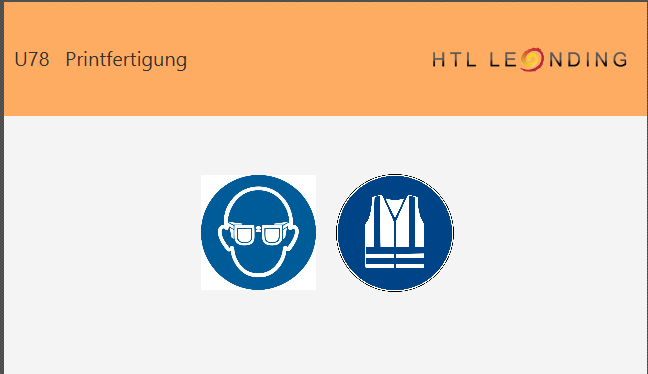
\includegraphics[width=0.45\textwidth]{images/views_examples/workshop_gebote_beispiel.PNG}
    \caption{Workshop view - example}
\end{figure}
\vspace{0,5 cm}
\textbf{Special rooms and events} \\
\\
Depending on the room, there will be information displayed about the current lesson/event/test taking place, accompanied by the room’s name (e.g. “Physiksaal”).\\
\\
There are currently 2 types of special rooms:
\begin{itemize}
\item The multipurpose hall (room number E26)
\item Rooms used for events like open-doors days
\end{itemize}
There are mostly events like presentations, project awards or even the oral final exam taking place. All these events can have the same interface. \\
\\
There is a variety of other events that are yearly taking place in our school. The most important events that need a special interface are:
\begin{itemize}
\item Open doors’ day
\item FIT (Firmeninformationstag)
\item Parent conference day: every year the students’ parents are invited to conferences with the teachers in order to talk about their children. Every teacher is in a room an has a schedule with all the parents that want to talk to him/her. This schedule can be digitalized and be put on the tablets.
\end{itemize}

Other events like Girls’ Day, IoT (lessons taking place on Saturdays) or the so-called “Schnupperprogrammieren” can also have the same interface as FIT. \\
\\

\textbf{Admin Page}

There already exists an admin interface made by a preliminary project. This admin interface is used to log in the tablets for the first time and to choose which room type has to be shown on each table. \\
If there is an event taking place in the school (e.g. Open Doors Day), a so-called “Event Mode” should be able to be started. Then the admin should be able to choose the tablets he needs for the events and choose between a variety of events. For each tablet, he will be able to insert the title of the event that is taking place in each room and, depending on the event, there will also be the possibility to add a description of the event.

\begin{figure}
    \centering
    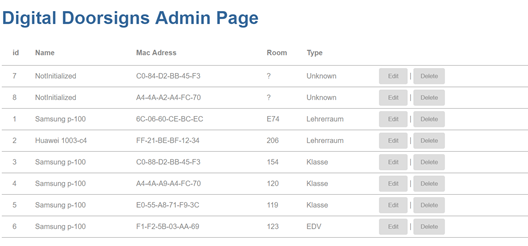
\includegraphics[width=0.75\textwidth]{images/views_examples/adminpage.png}
    \caption{Admin Page view}
\end{figure}

\vspace{0.5cm}
\textbf{Central view} \\
\\
By the entrance of our school we want a bigger display that will show
\begin{itemize}
\item current events (e.g. workshops) in our school and the rooms where they take place.
\end{itemize}
\end{explanation}

\section{Opportunities and Risks}
\begin{explanation}
The project has the following \textbf{opportunities}:
\begin{itemize}
    \item Teachers save time when searching for free rooms
    \item Classrooms that are taking tests are not disturbed during them
    \item Students searching for teachers know immediately where the teachers are by looking at their current location on the tablet
    \item When wanting to use a computer room, the weekly schedule will show on the table in order to see at which time the room is free
    \item People that are not familiar with our rooms can easily find what they search for. Furthermore our solution offers flexibility regarding the events that take place in our schools since we design multiple designs which can be chosen depending on the event.
\item More modern look of our school
\end{itemize}

\vspace{0.5cm}
The following \textbf{risks} are:
\begin{itemize}
    \item Vandalism – students can damage the tablets/E-Paper devices
    \item Hacking
    \item Power supply (Tablets consume a lot of energy. Also, in the case of power failure, the tablets/E-Paper won’t work)
    \item WebUntis has a clumsy user interface. This is the main reason why most teacher don’t like scheduling their events into WebUntis. Our solution will currently just sup-ports him/her in finding available rooms faster.
    \item Since we have over 100 rooms in our school, providing every classroom with a tablet can become pretty expensive
\end{itemize}

\vspace{0.5cm}
Potential \textbf{customers}: \\
Our school and other schools that like our solution and also use WebUntis.
\end{explanation}
\pagebreak
\section{Planning}

\textbf{Milestones:}

\begin{center}
\begin{tabular}{|l|l|}
\hline
Project Proposal & 25.10.2019 \\ \hline
Views examples for all rooms/events & 3.11.2019 \\ \hline
Poster (draft) with views for presentation scopes & 4.11.2019 \\ \hline
Ready poster for presentation scopes & 11.11.2019 \\ \hline
\end{tabular}    
\end{center}

\vspace{0.5cm}

\textbf{Needed resources:}
\begin{itemize}
    \item A WebUntis account
    \item Tablets
    \item E-Paper devices
    \item ESP32 Micro Controllers
\end{itemize}

\vspace{0.5cm}

\textbf{Team structure:}
\begin{center}
    \begin{tabular}{|l|l|}
    \hline
       Developer/ team leader  &  Gloria Sara Panturu\\ \hline
        Developer & Felix Bogengruber \\ \hline
        Developer & Belmin Coralic \\ \hline
        Developer & Janine Höllhuber \\ \hline
    \end{tabular}
\end{center}

\textbf{What needs to be done:}
\begin{itemize}
    \item Create an admin page for the E-Paper devices
    \item Update the current admin page in order to add support for the special events
    \item Create views for all the special events
    \item Create views for the workshop rooms
\end{itemize}
\end{document}
